% !TEX TS-program = XeLaTeX-shellescape
\documentclass[10pt, compress]{beamer}

\usetheme{m}

\usepackage{xcolor}
\usepackage{booktabs}
\usepackage[scale=2]{ccicons}
\usepackage{minted}
\usepackage{tikz}
\usemintedstyle{trac}
\newcounter{mycount}

\tikzset{
	mygrid/.pic={
		  
\draw[step=1cm,color=gray] (-2,-2) grid (3,3);
    \node[fill=cyan] at (-1.5,2.5) {};
    \node[fill=cyan] at (0.5,2.5) {};
    \node[fill=cyan] at (-.5,.5) {};
    \node[fill=cyan] at (2.5,.5) {};
    \node[fill=cyan] at (-1.5,2.5) {};
    \node[fill=cyan] at (1.5,-.5) {};
    \node[fill=cyan] at (-1.5,-1.5) {};

\setcounter{mycount}{1}
\foreach \y in {+2.6,+1.6,.6,-.4,-1.4}
  \foreach \x in {-1.6,-0.6,.4,1.4,2.4}
    \node at (\x,\y)[anchor=north west] {\tiny\arabic{mycount}\addtocounter{mycount}{1}};


	},
	popgrid/.pic = {
		
	\draw[step=1cm,color=gray] (-2,-2) grid (3,3);
   \node[fill=cyan] at (-1.5,2.5) {};
    \node[fill=cyan] at (-.5,.5) {};
     \node[fill=cyan] at (0.5,2.5) {};
    \node[fill=cyan] at (-1.5,2.5) {};
    \node[fill=cyan] at (2.5,.5) {};
    \node[fill=cyan] at (1.5,-.5) {};
    \node[fill=cyan] at (-1.5,-1.5) {};
    \node at (-1.5,1.5){40};
     \node at (-1.5,.5){40};
     \node at (-1.5,-.5){40};
     \node at (-.5,2.5){200};
     \node at (-.5,1.5){100};
     \node at (-.5,-.5){50};
     \node at (0.5,-.5){130};
      \node at (.5,.5){150};
       \node at (.5,1.5){150};
       \node at (1.5, 1.5){160};
       \node at (2.5, 1.5){20};
       \node at (2.5,2.5){30};
       \node at (1.5,2.5){200};
       \node at (1.5,.5){140};
       \node at (-.5,-1.5){60};
       \node at (.5,-1.5){70};
        \node at (1.5,-1.5){80};
         \node at (2.5,-1.5){40};
         \node at (2.5,-.5){80};
   
\setcounter{mycount}{1}
\foreach \y in {+2.6,+1.6,.6,-.4,-1.4}
  \foreach \x in {-1.6,-0.6,.4,1.4,2.4}
    \node at (\x,\y)[anchor=north west] {\tiny\arabic{mycount}\addtocounter{mycount}{1}};
		
	},
	bigexample/.pic = {
		
	\draw [step=0.5cm, very thin, color=black, solid] (0, 0) grid (7.5, 5);
	% row 1 pop
	\node at (0.25,4.75){\footnotesize 50};
	\node at (0.75,4.75){\footnotesize 55};
	\node at (1.75,4.75){\footnotesize 40};
	\node at (2.25,4.75){\footnotesize 60};
	\node at (2.75,4.75){\footnotesize 85};
	\node at (3.25,4.75){\footnotesize 65};
	\node at (3.75,4.75){\footnotesize 120};
	\node at (4.25,4.75){\footnotesize 105};
	\node at (4.75,4.75){\footnotesize 95};
	\node at (5.25,4.75){\footnotesize 85};
	\node at (6.25,4.75){\footnotesize 65};
	\node at (6.75,4.75){\footnotesize 45};
	% row 2 pop
	\node at (0.75,4.25){\footnotesize 50};
	\node at (1.25,4.25){\footnotesize 45};
	\node at (1.75,4.25){\footnotesize 60};
	\node at (2.25,4.25){\footnotesize 110};
	\node at (2.75,4.25){\footnotesize 120};
	\node at (3.25,4.25){\footnotesize 95};
	\node at (3.75,4.25){\footnotesize 110};
	\node at (4.75,4.25){\footnotesize 100};
	\node at (5.25,4.25){\footnotesize 65};
	\node at (5.75,4.25){\footnotesize 75};
	\node at (6.25,4.25){\footnotesize 40};
	\node at (6.75,4.25){\footnotesize 45};
	\node at (7.25,4.25){\footnotesize 30};
	% row 3 pop
	\node at (0.25,3.75){\footnotesize 80};
	\node at (0.75,3.75){\footnotesize 75};
	\node at (1.25,3.75){\footnotesize 55};
	\node at (1.75,3.75){\footnotesize 70};
	\node at (2.25,3.75){\footnotesize 105};
	\node at (2.75,3.75){\footnotesize 130};
	\node at (3.25,3.75){\footnotesize 115};
	\node at (4.25,3.75){\footnotesize 105};
	\node at (4.75,3.75){\footnotesize 115};
	\node at (5.25,3.75){\footnotesize 80};
	\node at (5.75,3.75){\footnotesize 50};
	\node at (6.25,3.75){\footnotesize 65};
	\node at (6.75,3.75){\footnotesize 50};
	% row 4 pop
	\node at (0.25,3.25){\footnotesize 165};
	\node at (1.25,3.25){\footnotesize 65};
	\node at (2.25,3.25){\footnotesize 65};
	\node at (2.75,3.25){\footnotesize 80};
	\node at (3.25,3.25){\footnotesize 95};
	\node at (3.75,3.25){\footnotesize 110};
	\node at (4.25,3.25){\footnotesize 105};
	\node at (5.25,3.25){\footnotesize 70};
	\node at (5.75,3.25){\footnotesize 55};
	\node at (6.25,3.25){\footnotesize 45};
	\node at (7.25,3.25){\footnotesize 25};
	% row 5 pop
	\node at (0.25,2.75){\footnotesize 225};
	\node at (0.75,2.75){\footnotesize 200};
	\node at (1.25,2.75){\footnotesize 70};
	\node at (1.75,2.75){\footnotesize 75};
	\node at (2.25,2.75){\footnotesize 100};
	\node at (3.25,2.75){\footnotesize 100};
	\node at (3.75,2.75){\footnotesize 105};
	\node at (4.25,2.75){\footnotesize 120};
	\node at (4.75,2.75){\footnotesize 105};
	\node at (5.25,2.75){\footnotesize 55};
	\node at (6.25,2.75){\footnotesize 20};
	\node at (6.75,2.75){\footnotesize 25};
	\node at (7.25,2.75){\footnotesize 15};
	% row 6 pop
	\node at (0.25,2.25){\footnotesize 250};
	\node at (0.75,2.25){\footnotesize 120};
	\node at (1.75,2.25){\footnotesize 85};
	\node at (2.25,2.25){\footnotesize 105};
	\node at (2.75,2.25){\footnotesize 100};
	\node at (3.25,2.25){\footnotesize 110};
	\node at (3.75,2.25){\footnotesize 70};
	\node at (4.25,2.25){\footnotesize 80};
	\node at (4.75,2.25){\footnotesize 70};
	\node at (5.25,2.25){\footnotesize 65};
	\node at (5.75,2.25){\footnotesize 50};
	\node at (6.25,2.25){\footnotesize 15};
	\node at (6.75,2.25){\footnotesize 5};
	\node at (7.25,2.25){\footnotesize 10};
	% row 7 pop
	\node at (0.25,1.75){\footnotesize 200};
	\node at (0.75,1.75){\footnotesize 100};
	\node at (1.25,1.75){\footnotesize 180};
	\node at (1.75,1.75){\footnotesize 155};
	\node at (2.25,1.75){\footnotesize 125};
	\node at (2.75,1.75){\footnotesize 105};
	\node at (3.25,1.75){\footnotesize 80};
	\node at (4.25,1.75){\footnotesize 95};
	\node at (4.75,1.75){\footnotesize 75};
	\node at (5.25,1.75){\footnotesize 40};
	\node at (5.75,1.75){\footnotesize 45};
	\node at (6.25,1.75){\footnotesize 35};
	\node at (7.25,1.75){\footnotesize 15};
	% row 8 pop
	\node at (0.25,1.25){\footnotesize 250};
	\node at (1.75,1.25){\footnotesize 145};
	\node at (2.75,1.25){\footnotesize 235};
	\node at (3.25,1.25){\footnotesize 100};
	\node at (3.75,1.25){\footnotesize 80};
	\node at (4.25,1.25){\footnotesize 135};
	\node at (4.75,1.25){\footnotesize 95};
	\node at (5.25,1.25){\footnotesize 70};
	\node at (6.25,1.25){\footnotesize 50};
	\node at (6.75,1.25){\footnotesize 45};
	\node at (7.25,1.25){\footnotesize 20};
	% row 9 pop
	\node at (0.25,0.75){\footnotesize 300};
	\node at (1.25,0.75){\footnotesize 265};
	\node at (1.75,0.75){\footnotesize 205};
	\node at (2.25,0.75){\footnotesize 235};
	\node at (2.75,0.75){\footnotesize 505};
	\node at (3.25,0.75){\footnotesize 500};
	\node at (3.75,0.75){\footnotesize 245};
	\node at (4.25,0.75){\footnotesize 175};
	\node at (4.75,0.75){\footnotesize 80};
	\node at (5.25,0.75){\footnotesize 85};
	\node at (5.75,0.75){\footnotesize 65};
	\node at (6.25,0.75){\footnotesize 30};
	\node at (7.25,0.75){\footnotesize 25};
	% row 10 pop
	\node at (0.25,0.25){\footnotesize 305};
	\node at (0.75,0.25){\footnotesize 255};
	\node at (1.25,0.25){\footnotesize 275};
	\node at (1.75,0.25){\footnotesize 215};
	\node at (2.25,0.25){\footnotesize 225};
	\node at (2.75,0.25){\footnotesize 400};
	\node at (3.25,0.25){\footnotesize 405};
	\node at (3.75,0.25){\footnotesize 410};
	\node at (4.25,0.25){\footnotesize 500};
	\node at (4.75,0.25){\footnotesize 305};
	\node at (5.75,0.25){\footnotesize 45};
	\node at (6.25,0.25){\footnotesize 50};
	\node at (6.75,0.25){\footnotesize 40};
	\node at (7.25,0.25){\footnotesize 30};

	% candidate parcels
	\filldraw[fill=cyan, draw=black] (7, 4.5) rectangle (7.5, 5);
	\filldraw[fill=cyan, draw=black] (5.5, 4.5) rectangle (6, 5);
	\filldraw[fill=cyan, draw=black] (1, 4.5) rectangle (1.5, 5);
	\filldraw[fill=cyan, draw=black] (0, 4) rectangle (0.5, 4.5);
	\filldraw[fill=cyan, draw=black] (4, 4) rectangle (4.5, 4.5);
	\filldraw[fill=cyan, draw=black] (3.5, 3.5) rectangle (4, 4);
	\filldraw[fill=cyan, draw=black] (7, 3.5) rectangle (7.5, 4);
	\filldraw[fill=cyan, draw=black] (0.5, 3) rectangle (1, 3.5);
	\filldraw[fill=cyan, draw=black] (1.5, 3) rectangle (2, 3.5);
	\filldraw[fill=cyan, draw=black] (4.5, 3) rectangle (5, 3.5);
	\filldraw[fill=cyan, draw=black] (6.5, 3) rectangle (7, 3.5);
	\filldraw[fill=cyan, draw=black] (2.5, 2.5) rectangle (3, 3);
	\filldraw[fill=cyan, draw=black] (5.5, 2.5) rectangle (6, 3);
	\filldraw[fill=cyan, draw=black] (1, 2) rectangle (1.5, 2.5);
	\filldraw[fill=cyan, draw=black] (3.5, 1.5) rectangle (4, 2);
	\filldraw[fill=cyan, draw=black] (6.5, 1.5) rectangle (7, 2);
	\filldraw[fill=cyan, draw=black] (0.5, 1) rectangle (1, 1.5);
	\filldraw[fill=cyan, draw=black] (1, 1) rectangle (1.5, 1.5);
	\filldraw[fill=cyan, draw=black] (2, 1) rectangle (2.5, 1.5);
	\filldraw[fill=cyan, draw=black] (5.5, 1) rectangle (6, 1.5);
	\filldraw[fill=cyan, draw=black] (0.5, 0.5) rectangle (1, 1);
	\filldraw[fill=cyan, draw=black] (6.5, 0.5) rectangle (7, 1);
	\filldraw[fill=cyan, draw=black] (5, 0) rectangle (5.5, 0.5);
	
	}
	}



\title{Locating Parks with a Multiobjective Optimization Method}
\subtitle{}
\date{\today}
\author{Alan Peral \\ Professor Shahriari}
\institute{Pomona College}


%
% /Library/TeX/texbin:/Users/Boby/miniconda3/bin
%
\begin{document}

\maketitle
\section{The Problem}
%\begin{frame}[fragile]
  %\frametitle{}

	%\begin{block}{What does this mean?}
	%\end{block}

%\end{frame}

\begin{frame}{Bogot\'{a}, Colombia}
  \begin{itemize}[<+- | alert@+>]
    \item Large city % population expected to reach 10 million by 2025, implemented changes to recover public spaces and improve public parks
    \item Sports and recreation master plan % developed in 2006, indicated that by 2019 city must reach a min level of 2.71 m^2 of neighborhood park area per resident.
    \item Instituto Distrital de Recreaci\'{o}n y Deporte % Recreation and Sports Institute of Bogota had to implement master plan 
    \item A challenge % execute construction of numerous new parks and revitalize dilapidated public spaces in a manner that balanced the differing geographic, social, and economic needs of city 
   \end{itemize}
\end{frame}

\plain{Bogot\'{a}, Colombia}{\vspace{-2em}\begin{center}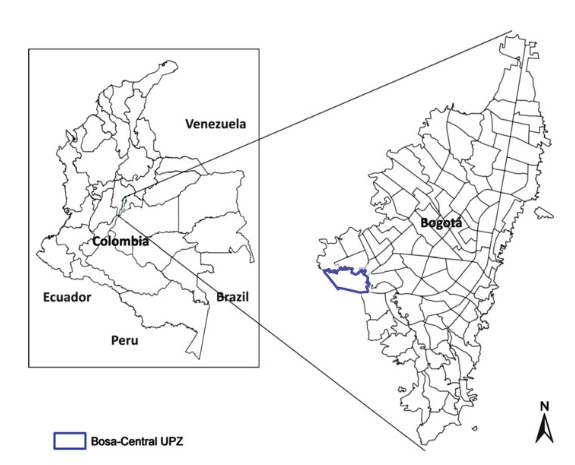
\includegraphics[width=14em]{images/bosa-central.png}\end{center}}

\plain{Bogot\'{a}, Colombia}{\vspace{-2em}\begin{center}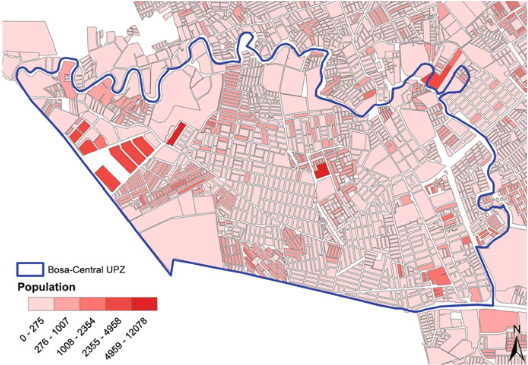
\includegraphics[width=14em]{images/pop-distrib.png}\end{center}}



\begin{frame}{Park Selection }
  \begin{itemize}[<+- | alert@+>]
    \item Candidate parcels % Empty lots throughout the city on which parks could be built
    \item Number of beneficiaries 
    \item Geographic coverage
    \item Sidewalk and road accessibility
    \item Positive and negative externalities provided by nearby facilities
    \item Construction and parcel acquisition cost
    \item Competing objectives
    \item Community Based Operations Research
   \end{itemize}
\end{frame}





%%%%%%%%%%%%
%%%%%%%%%%%% Talk about problem more at length here!!!!!!!!!!!!
%%%%%%%%%%%%
\section{The Groundwork} 
%%%
%%
% LINEAR PROGRAM
%%
%%%

\begin{frame}{Linear Program}

  \begin{itemize}[<+- | alert@+>]
    \item Mid-20th century development % since its development, it has been used to save millions of dollars for many businesses with its use in other sectors of society spreading quickly, dozens of textbooks and hundreds of articles have been published about it. it's been huge!
    \item Limited resources % allocating limited resources among competing activities in a best possible (optimal) way
    \item Competing activities
    \item Optimal 
    \item Linear model %  all mathematical functions in this model must be linear functions, and the word program here refers not to computers but functions as a synonym for planning
    \item Planning activities % thus we can conclude that a linear program helps plan activities
   \end{itemize}
\end{frame}

\begin{frame}{Linear Program}

\begin{alignat*}{2}
  & \text{Maximize: } & & Z = c_1x_1 + c_2x_2 + \dots + c_nx_n, \\
   & \text{subject to: }& \quad & a_{11}x_1 + a_{12}x_2 + \dots + a_{1n}x_n \leq b_1 \\
   & & &  a_{21}x_1 + a_{22}x_2 + \dots + a_{2n}x_n \leq b_2 \\  
   & &  & \quad \quad \quad \quad \quad \quad \quad \vdots \\
   & & &  a_{m1}x_1 + a_{m2}x_2 + \dots + a_{mn}x_n \leq b_m, \\   
   & & & x_1 \geq 0, x_2 \geq 0, \dots ,  x_n \geq 0
     \end{alignat*}

\end{frame}

\begin{frame}{Linear Program}

\begin{alignat*}{2}
  & \color{orange}\text{Maximize: } & & \color{orange}Z = c_1x_1 + c_2x_2 + \dots + c_nx_n, \\
   & \text{subject to: }& \quad & a_{11}x_1 + a_{12}x_2 + \dots + a_{1n}x_n \leq b_1 \\
   & & &  a_{21}x_1 + a_{22}x_2 + \dots + a_{2n}x_n \leq b_2 \\  
   & &  & \quad \quad \quad \quad \quad \quad \quad \vdots \\
   & & &  a_{m1}x_1 + a_{m2}x_2 + \dots + a_{mn}x_n \leq b_m, \\   
   & & & x_1 \geq 0, x_2 \geq 0, \dots ,  x_n \geq 0
     \end{alignat*}

\end{frame}

\begin{frame}{Linear Program}
\color{orange}
\begin{alignat*}{2}
   & \color{black} \text{Maximize: } & &\color{black} Z = c_1x_1 + c_2x_2 + \dots + c_nx_n, \\
   & \text{subject to: }& \quad & a_{11}x_1 + a_{12}x_2 + \dots + a_{1n}x_n \leq b_1 \\
   & & &  a_{21}x_1 + a_{22}x_2 + \dots + a_{2n}x_n \leq b_2 \\  
   & &  & \quad \quad \quad \quad \quad \quad \quad \vdots \\
   & & &  a_{m1}x_1 + a_{m2}x_2 + \dots + a_{mn}x_n \leq b_m, \\   
   & & & \color{black} x_1 \geq 0, x_2 \geq 0, \dots ,  x_n \geq 0
     \end{alignat*}

\end{frame}

\begin{frame}{Linear Program}

\begin{alignat*}{2}
  & \text{Maximize: } & & Z = c_1x_1 + c_2x_2 + \dots + c_nx_n, \\
   & \text{subject to: }& \quad & a_{11}x_1 + a_{12}x_2 + \dots + a_{1n}x_n \leq b_1 \\
   & & &  a_{21}x_1 + a_{22}x_2 + \dots + a_{2n}x_n \leq b_2 \\  
   & &  & \quad \quad \quad \quad \quad \quad \quad \vdots \\
   & & &  a_{m1}x_1 + a_{m2}x_2 + \dots + a_{mn}x_n \leq b_m, \\   
   & & & \color{orange}  x_1 \geq 0, x_2 \geq 0, \dots ,  x_n \geq 0
     \end{alignat*}

\end{frame}



%\section{The literature}

%\begin{frame}{Multiobjective methods}
%Talk about multiobjective problem, solution methods, etc.
%\end{frame}

%\begin{frame}{Facility location problems}
%Talk about relevant stuff.
%\end{frame}

%\begin{frame}{Purpose}
%Here talk about how things usually are about maximizing profits, and it's rather simple to minimize or maximize a dollar amount, but things get complicated when you have to consider multiple conflicting optimization goals. In community-based, public sector and nonprofit oriented OR, these things may be harder to solve
%\end{frame}




%%%%%%%%%%%%
%%%%%%%%%%%% should define the variables before diving into LP
%%%%%%%%%%%%
\section{The Model}

\plain{Bogot\'{a}, Colombia}{\vspace{-2em}\begin{center}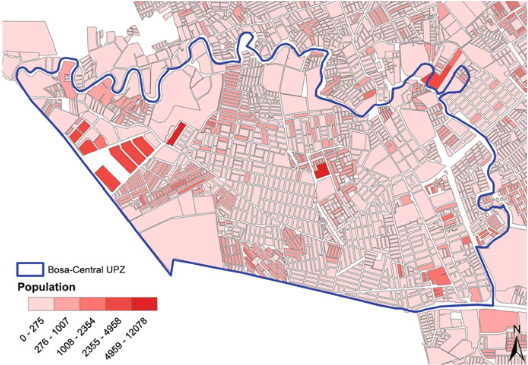
\includegraphics[width=14em]{images/pop-distrib.png}\end{center}}

\begin{frame}[fragile]
\frametitle{Simplifying Assumptions}
\begin{itemize}[<+- | alert@+>]
\item $m \times n$ grid
\item One block $=$ one square
\item Every block same size
\item Service area of a block is all bordering blocks (excluding candidate parcels)
\end{itemize}
\end{frame}

\begin{frame}[fragile]
\frametitle{Objective functions}
\begin{itemize}[<+- | alert@+>]
\item Maximize geographical coverage
\item[] $f_1$ 
\item Maximize people serviced
\item[] $f_3$
\end{itemize}
\end{frame}

\begin{frame}[fragile]
  \frametitle{Example}
  \begin{center}
  \begin{tikzpicture}[every node/.style={minimum size=1cm-\pgflinewidth}]
  \pic{mygrid};
\end{tikzpicture}
 \end{center}
This is our $5\times5$ grid city

\end{frame}


\begin{frame}[fragile]
  \frametitle{Example}
  \begin{center}
 \begin{tikzpicture}[every node/.style={minimum size=1cm-\pgflinewidth}]
  \pic{mygrid};
\end{tikzpicture}
\end{center}
\begin{itemize}
\item Candidate parcels
\end{itemize}
\end{frame}

\begin{frame}[fragile]
  \frametitle{Example}
  \begin{center}
 \begin{tikzpicture}[every node/.style={minimum size=1cm-\pgflinewidth}]
  \pic{mygrid};
\end{tikzpicture}
\end{center}
\begin{itemize}
\item Candidate parcels: $\mathcal{I} = \{1,3,12,15,19,21\}$
\end{itemize}
\end{frame}

\begin{frame}[fragile]
  \frametitle{Example}
  \begin{center}
 \begin{tikzpicture}[every node/.style={minimum size=1cm-\pgflinewidth}]
  \pic{mygrid};
\end{tikzpicture}
\end{center}
\begin{itemize}
\item Candidate parcels: $\mathcal{I} = \{1,3,12,15,19,21\}$; \;$y_i, \; i \in \mathcal{I}$
\end{itemize}
\end{frame}

\begin{frame}[fragile]
  \frametitle{Example}
  \begin{center}
 \begin{tikzpicture}[every node/.style={minimum size=1cm-\pgflinewidth}]
  \pic{mygrid};
\end{tikzpicture}
\end{center}
\begin{itemize}
\item Candidate parcels: $\mathcal{I} = \{1,3,12,15,19,21\}$; \; $\color{orange} y_{19} = 1$
\end{itemize}
\end{frame}

\begin{frame}[fragile]
  \frametitle{Example}
  \begin{center}
 \begin{tikzpicture}[every node/.style={minimum size=1cm-\pgflinewidth}]
  \pic{mygrid};
\end{tikzpicture}
\end{center}
\begin{block}{Which candidate parcel will maximize geographical coverage?}
\end{block}
\end{frame}

\begin{frame}[fragile]
  \frametitle{Example}
  \begin{center}
 \begin{tikzpicture}[every node/.style={minimum size=1cm-\pgflinewidth}]
  \pic{mygrid};
\end{tikzpicture}
\end{center}
\begin{block}{Which candidate parcel will maximize geographical coverage?}
\alert{Candidate 12}
\end{block}
\end{frame}

\begin{frame}[fragile]
  \frametitle{Example}
  \begin{center}
 \begin{tikzpicture}[every node/.style={minimum size=1cm-\pgflinewidth}]
  \pic{mygrid};
\end{tikzpicture}
\end{center}
\begin{itemize}
\item $\mathcal{J} = \{2,4,6,7, \dots, 23,24,25\}$
\end{itemize}
\end{frame}

\begin{frame}[fragile]
  \frametitle{Example}
  \begin{center}
 \begin{tikzpicture}[every node/.style={minimum size=1cm-\pgflinewidth}]
  \pic{mygrid};
\end{tikzpicture}
\end{center}
\begin{itemize}
\item $\mathcal{J} = \{2,4,6,7, \dots, 23,24,25\}$, the set of all blocks that would benefit from the construction of a new park
\end{itemize}
\end{frame}

\begin{frame}[fragile]
  \frametitle{Example}
  \begin{center}
 \begin{tikzpicture}[every node/.style={minimum size=1cm-\pgflinewidth}]
  \pic{mygrid};
\end{tikzpicture}
\end{center}
\begin{itemize}
\item $\mathcal{J} = \{2,4,6,7, \dots, 23,24,25\}$
\item $z_j$, \; $j \in \mathcal{J}$, $1$ if block $j$ is serviced by a selected parcel, 0 otherwise
\end{itemize}
\end{frame}

\begin{frame}[fragile]
  \frametitle{Example}
  \begin{center}
 \begin{tikzpicture}[every node/.style={minimum size=1cm-\pgflinewidth}]
  \pic{mygrid};
\end{tikzpicture}
\end{center}
\begin{itemize}
\item $\mathcal{J} = \{2,4,6,7, \dots, 23,24,25\}$
\item $\color{orange} z_2 = z_6 = z_7 = 1, \quad z_4 = z_8 = z_9 = \dots = z_{24} = z_{25} = 0$
\end{itemize}
\end{frame}

\begin{frame}[fragile]
  \frametitle{Example}
  \begin{center}
 \begin{tikzpicture}[every node/.style={minimum size=1cm-\pgflinewidth}]
  \pic{mygrid};
\end{tikzpicture}
\end{center}
\begin{itemize}
\item $\mathcal{J} = \{2,4,6,7, \dots, 23,24,25\}$
\item $z_j$, \; $j \in \mathcal{J}$, takes on value $1$ if block $j$ is serviced by a selected parcel, 0 otherwise
\item $\mathcal{W}_j$, \; $j \in \mathcal{J}$,  the set of candidate parcels that serve block $j$
\end{itemize}
\end{frame}

\begin{frame}[fragile]
  \frametitle{Example}
  \begin{center}
 \begin{tikzpicture}[every node/.style={minimum size=1cm-\pgflinewidth}]
  \pic{mygrid};
\end{tikzpicture}
\end{center}
\begin{itemize}
\item $\mathcal{J} = \{2,4,6,7, \dots, 23,24,25\}$
\item $z_j$, \; $j \in \mathcal{J}$
\item $\color{orange}\mathcal{W}_7 = \{1,3,12\}$
\end{itemize}
\end{frame}

\begin{frame}[fragile]
\frametitle{LP to Maximize Geographical Coverage}
\noindent\fbox{%
    \parbox{\textwidth}{%
        {\scriptsize $z_j = 1$ if block $j$ is serviced by a selected parcel, 0 otherwise \\
$y_i = 1$ if candidate parcel $i$ is selected to become a park, 0 otherwise}
    }%
}
\begin{align*}
\textrm{max } f_1 &= \sum_{j \in \mathcal{J}} z_j \\
\textrm{subject to } z_j &\leq \sum_{i \in \mathcal{W}_j} y_i, \quad j \in \mathcal{J}\\
\left|\mathcal{W}_j\right|z_j &\geq \sum_{i \in \mathcal{W}_j} y_i, \quad j \in \mathcal{J} \\
z_j &\in \{0,1\}, \quad \; j \in \mathcal{J} \\
y_i &\in \{0,1\}, \quad \; i \in \mathcal{I}
\end{align*}
\end{frame}

\begin{frame}[fragile]
\frametitle{LP to Maximize Geographical Coverage}
\noindent\fbox{%
    \parbox{\textwidth}{%
        {\scriptsize $z_j = 1$ if block $j$ is serviced by a selected parcel, 0 otherwise \\
$y_i = 1$ if candidate parcel $i$ is selected to become a park, 0 otherwise}
    }%
}
\begin{align*}\color{orange}
\textrm{max } f_1 &\color{orange}= \sum_{j \in \mathcal{J}} z_j \\
\textrm{subject to } z_j &\leq \sum_{i \in \mathcal{W}_j} y_i, \quad j \in \mathcal{J}\\
\left|\mathcal{W}_j\right|z_j &\geq \sum_{i \in \mathcal{W}_j} y_i, \quad j \in \mathcal{J} \\
z_j &\in \{0,1\}, \quad \; j \in \mathcal{J} \\
y_i &\in \{0,1\}, \quad \; i \in \mathcal{I}
\end{align*}
\end{frame}

\begin{frame}[fragile]
\frametitle{LP to Maximize Geographical Coverage}
\noindent\fbox{%
    \parbox{\textwidth}{%
        {\scriptsize $z_j = 1$ if block $j$ is serviced by a selected parcel, 0 otherwise \\
$y_i = 1$ if candidate parcel $i$ is selected to become a park, 0 otherwise}
    }%
}
\begin{align*}
\textrm{max } f_1 &= \sum_{j \in \mathcal{J}} z_j \\
\color{orange}\textrm{subject to } z_j &\color{orange} \leq \sum_{i \in \mathcal{W}_j} y_i, \quad j \in \mathcal{J}\\
\left|\mathcal{W}_j\right|z_j &\geq \sum_{i \in \mathcal{W}_j} y_i, \quad j \in \mathcal{J} \\
z_j &\in \{0,1\}, \quad \; j \in \mathcal{J} \\
y_i &\in \{0,1\}, \quad \; i \in \mathcal{I}
\end{align*}
\end{frame}

\begin{frame}[fragile]
\frametitle{LP to Maximize Geographical Coverage}
\noindent\fbox{%
    \parbox{\textwidth}{%
        {\scriptsize $z_j = 1$ if block $j$ is serviced by a selected parcel, 0 otherwise \\
$y_i = 1$ if candidate parcel $i$ is selected to become a park, 0 otherwise}
    }%
}
\begin{align*}
\textrm{max } f_1 &= \sum_{j \in \mathcal{J}} z_j \\
\textrm{subject to } z_j &\leq \sum_{i \in \mathcal{W}_j} y_i, \quad j \in \mathcal{J}\\
\color{orange} \left|\mathcal{W}_j\right|z_j & \color{orange} \geq \sum_{i \in \mathcal{W}_j} y_i, \quad j \in \mathcal{J} \\
z_j &\in \{0,1\}, \quad \; j \in \mathcal{J} \\
y_i &\in \{0,1\}, \quad \; i \in \mathcal{I}
\end{align*}
\end{frame}

\begin{frame}[fragile]
\frametitle{LP to Maximize Geographical Coverage}
\noindent\fbox{%
    \parbox{\textwidth}{%
        {\scriptsize $z_j = 1$ if block $j$ is serviced by a selected parcel, 0 otherwise \\
$y_i = 1$ if candidate parcel $i$ is selected to become a park, 0 otherwise}
    }%
}
\begin{align*}
\textrm{max } f_1 &= \sum_{j \in \mathcal{J}} z_j \\
\textrm{subject to } z_j &\leq \sum_{ i \in \mathcal{W}_j} y_i, \quad \color{orange} j \in \mathcal{J}\\
\left|\mathcal{W}_j\right|z_j &\geq \sum_{i \in \mathcal{W}_j} y_i, \quad \color{orange} j \in \mathcal{J} \\
z_j &\in \{0,1\}, \quad \; j \in \mathcal{J} \\
y_i &\in \{0,1\}, \quad \; i \in \mathcal{I}
\end{align*}
\end{frame}

\begin{frame}[fragile]
\frametitle{LP to Maximize Geographical Coverage}
\noindent\fbox{%
    \parbox{\textwidth}{%
        {\scriptsize $z_j = 1$ if block $j$ is serviced by a selected parcel, 0 otherwise \\
$y_i = 1$ if candidate parcel $i$ is selected to become a park, 0 otherwise}
    }%
}
\begin{align*}
\textrm{max } f_1 &= \sum_{j \in \mathcal{J}} z_j \\
\textrm{subject to } z_j &\leq \sum_{i \in \mathcal{W}_j} y_i, \quad j \in \mathcal{J}\\
\left|\mathcal{W}_j\right|z_j &\geq \sum_{i \in \mathcal{W}_j} y_i, \quad j \in \mathcal{J} \\
\color{orange} z_j &\color{orange} \in \{0,1\}, \quad \; j \in \mathcal{J} \\
\color{orange} y_i &\color{orange} \in \{0,1\}, \quad \; i \in \mathcal{I}
\end{align*}
\end{frame}

\begin{frame}[fragile]
\frametitle{LP to Maximize Geographical Coverage}
\noindent\fbox{%
    \parbox{\textwidth}{%
        {\scriptsize $z_j = 1$ if block $j$ is serviced by a selected parcel, 0 otherwise \\
$y_i = 1$ if candidate parcel $i$ is selected to become a park, 0 otherwise}
    }%
}
\begin{align*}
\textrm{max } f_1 &= \sum_{j \in \mathcal{J}} z_j \\
\textrm{subject to } z_j &\leq \sum_{i \in \mathcal{W}_j} y_i, \quad j \in \mathcal{J}\\
\left|\mathcal{W}_j\right|z_j &\geq \sum_{i \in \mathcal{W}_j} y_i, \quad j \in \mathcal{J} \\
\color{orange} p_{max} & \color{orange} \geq \sum_{i \in \mathcal{I}} y_i  \\
z_j &\in \{0,1\}, \quad \; j \in \mathcal{J} \\
y_i &\in \{0,1\}, \quad \; i \in \mathcal{I}
\end{align*}
\end{frame}


%%%%%%%%%%%%%
\begin{frame}[fragile]
\frametitle{Switching the Objective}
\begin{center}
\begin{tikzpicture}[every node/.style={minimum size=1cm-\pgflinewidth}]
  \pic{popgrid};
\end{tikzpicture}
\end{center}
\end{frame}


\begin{frame}[fragile]
\frametitle{Switching the Objective}
\begin{center}
\begin{tikzpicture}[every node/.style={minimum size=1cm-\pgflinewidth}]
  \pic{popgrid};
\end{tikzpicture}
\end{center}
\begin{block}{Which candidate parcel will maximize the number of beneficiaries?}
\end{block}
\end{frame}

\begin{frame}[fragile]
\frametitle{Switching the Objective}
\begin{center}
\begin{tikzpicture}[every node/.style={minimum size=1cm-\pgflinewidth}]
  \pic{popgrid};
\end{tikzpicture}
\end{center}
\begin{block}{Which candidate parcel will maximize the number of beneficiaries?}
\end{block}
\alert{$p_i$, \; $i \in \mathcal{I}$}
\end{frame}

\begin{frame}[fragile]
\frametitle{Both Objectives}
\begin{center}
\begin{tikzpicture}[every node/.style={minimum size=1cm-\pgflinewidth}]
  \pic{popgrid};
\end{tikzpicture}
\end{center}
\begin{block}{Which candidate parcel will maximize the number of beneficiaries and the geographic coverage?}
\end{block}
\end{frame}



\section{The Solution Strategy}

\begin{frame}[fragile]
\frametitle{Multiobjective}
\begin{itemize}
\item Maximize geographic coverage
\end{itemize}
\end{frame}

\begin{frame}[fragile]
\frametitle{Multiobjective}
\begin{itemize}
\item Maximize geographic coverage
\item Maximize number of beneficiaries
\end{itemize}
\end{frame}

\begin{frame}[fragile]
\frametitle{Multiobjective}
\begin{align*}
\textrm{max } f_1 &= \sum_{j \in \mathcal{J}} z_j \\
\textrm{max } f_3 &= \sum_{i \in \mathcal{I}} p_iy_i \\
\textrm{subject to } z_j &\leq \sum_{i \in \mathcal{W}_j} y_i, j \in \mathcal{J}\\
\left|\mathcal{W}_j\right|z_j &\geq \sum_{i \in \mathcal{W}_j} y_i, j \in \mathcal{J} \\
p_{max} &\geq \sum_{i \in \mathcal{I}} y_i  \\
z_j &\in \{0,1\}, j \in \mathcal{J} \\
y_i &\in \{0,1\}, i \in \mathcal{I}
\end{align*}
\end{frame}

\begin{frame}[fragile]
\frametitle{Multiobjective}
\begin{columns}[onlytextwidth]
\column{0.5\textwidth}
\begin{align*}
\textrm{max } f_1 &= \sum_{j \in \mathcal{J}} z_j \\
\textrm{subject to } z_j &\leq \sum_{i \in \mathcal{W}_j} y_i, j \in \mathcal{J}\\
\left|\mathcal{W}_j\right|z_j &\geq \sum_{i \in \mathcal{W}_j} y_i, j \in \mathcal{J} \\
p_{max} &\geq \sum_{i \in \mathcal{I}} y_i  \\
z_j &\in \{0,1\}, j \in \mathcal{J} \\
y_i &\in \{0,1\}, i \in \mathcal{I}
\end{align*}
\column{0.5\textwidth}
\begin{align*}
\textrm{max } f_3 &= \sum_{i \in \mathcal{I}} p_iy_i \\
\textrm{subject to } z_j &\leq \sum_{i \in \mathcal{W}_j} y_i, j \in \mathcal{J}\\
\left|\mathcal{W}_j\right|z_j &\geq \sum_{i \in \mathcal{W}_j} y_i, j \in \mathcal{J} \\
p_{max} &\geq \sum_{i \in \mathcal{I}} y_i  \\
z_j &\in \{0,1\}, j \in \mathcal{J} \\
y_i &\in \{0,1\}, i \in \mathcal{I}
\end{align*}
\end{columns}
\end{frame}

\begin{frame}[fragile]
\frametitle{Multiobjective}
\begin{columns}[onlytextwidth]
\column{0.5\textwidth}
\begin{align*}
\textrm{max } f_1 &= \sum_{j \in \mathcal{J}} z_j \\
\textrm{subject to } z_j &\leq \sum_{i \in \mathcal{W}_j} y_i, j \in \mathcal{J}\\
\left|\mathcal{W}_j\right|z_j &\geq \sum_{i \in \mathcal{W}_j} y_i, j \in \mathcal{J} \\
p_{max} &\geq \sum_{i \in \mathcal{I}} y_i  \\
z_j &\in \{0,1\}, j \in \mathcal{J} \\
y_i &\in \{0,1\}, i \in \mathcal{I} \\
& \alert{f_1^*}
\end{align*}
\column{0.5\textwidth}
\begin{align*}
\textrm{max } f_3 &= \sum_{i \in \mathcal{I}} p_iy_i \\
\textrm{subject to } z_j &\leq \sum_{i \in \mathcal{W}_j} y_i, j \in \mathcal{J}\\
\left|\mathcal{W}_j\right|z_j &\geq \sum_{i \in \mathcal{W}_j} y_i, j \in \mathcal{J} \\
p_{max} &\geq \sum_{i \in \mathcal{I}} y_i  \\
z_j &\in \{0,1\}, j \in \mathcal{J} \\
y_i &\in \{0,1\}, i \in \mathcal{I} \\
&\alert{f_3^*}
\end{align*}
\end{columns}
\begin{center}
\end{center}
\end{frame}

\begin{frame}[fragile]
\frametitle{Multiobjective}
\begin{columns}[onlytextwidth]
\column{0.5\textwidth}
\begin{align*}
\textrm{max } f_1 &= \sum_{j \in \mathcal{J}} z_j \\
\textrm{subject to } z_j &\leq \sum_{i \in \mathcal{W}_j} y_i, j \in \mathcal{J}\\
\left|\mathcal{W}_j\right|z_j &\geq \sum_{i \in \mathcal{W}_j} y_i, j \in \mathcal{J} \\
p_{max} &\geq \sum_{i \in \mathcal{I}} y_i  \\
z_j &\in \{0,1\}, j \in \mathcal{J} \\
y_i &\in \{0,1\}, i \in \mathcal{I} \\
\end{align*}
\column{0.5\textwidth}
\begin{align*}
\textrm{max } f_3 &= \sum_{i \in \mathcal{I}} p_iy_i \\
\textrm{subject to } z_j &\leq \sum_{i \in \mathcal{W}_j} y_i, j \in \mathcal{J}\\
\left|\mathcal{W}_j\right|z_j &\geq \sum_{i \in \mathcal{W}_j} y_i, j \in \mathcal{J} \\
p_{max} &\geq \sum_{i \in \mathcal{I}} y_i  \\
z_j &\in \{0,1\}, j \in \mathcal{J} \\
y_i &\in \{0,1\}, i \in \mathcal{I}
\end{align*}
\end{columns}
\begin{center}
\alert{$f_1^* = 8 \textrm{ blocks} \quad \quad \quad \quad \quad \quad \quad \quad \quad \quad \quad \quad f_3^* $}
\end{center}
\end{frame}

\begin{frame}[fragile]
\frametitle{Multiobjective}
\begin{columns}[onlytextwidth]
\column{0.5\textwidth}
\begin{align*}
\textrm{max } f_1 &= \sum_{j \in \mathcal{J}} z_j \\
\textrm{subject to } z_j &\leq \sum_{i \in \mathcal{W}_j} y_i, j \in \mathcal{J}\\
\left|\mathcal{W}_j\right|z_j &\geq \sum_{i \in \mathcal{W}_j} y_i, j \in \mathcal{J} \\
p_{max} &\geq \sum_{i \in \mathcal{I}} y_i  \\
z_j &\in \{0,1\}, j \in \mathcal{J} \\
y_i &\in \{0,1\}, i \in \mathcal{I}
\end{align*}
\column{0.5\textwidth}
\begin{align*}
\textrm{max } f_3 &= \sum_{i \in \mathcal{I}} p_iy_i \\
\textrm{subject to } z_j &\leq \sum_{i \in \mathcal{W}_j} y_i, j \in \mathcal{J}\\
\left|\mathcal{W}_j\right|z_j &\geq \sum_{i \in \mathcal{W}_j} y_i, j \in \mathcal{J} \\
p_{max} &\geq \sum_{i \in \mathcal{I}} y_i  \\
z_j &\in \{0,1\}, j \in \mathcal{J} \\
y_i &\in \{0,1\}, i \in \mathcal{I}
\end{align*}
\end{columns}
\begin{center}
\quad \quad \quad \quad \alert{$f_1^* = 8 \textrm{ blocks,} \quad \quad \quad \quad \quad \quad \quad \quad \quad \quad f_3^* = 810 \textrm{ people}$}
\end{center}
\end{frame}

\begin{frame}[fragile]
\frametitle{Compromise Threshold}
\begin{itemize}[<+- | alert@+>]
\item compromise threshold: $(1-\alpha_k)$
\item $\alpha_k$ maximum acceptable deterioration for objective $k$
\item $k=1,3$
\item $\alpha_1$ = 40\% means objective function 1 must be at least $60\%$ as optimal as the solution acquired in isolation
\end{itemize}
\end{frame}

\begin{frame}[fragile]
\begin{align*}
\textrm{max } f_3 &= \sum_{i \in \mathcal{I}} p_iy_i \\
\textrm{subject to } z_j &\leq \sum_{i \in \mathcal{W}_j} y_i, j \in \mathcal{J}\\
\left|\mathcal{W}_j\right|z_j &\geq \sum_{i \in \mathcal{W}_j} y_i, j \in \mathcal{J} \\
p_{max} &\geq \sum_{i \in \mathcal{I}} y_i  \\
\color{orange} \sum_{j \in \mathcal{J}} z_j & \color{orange} \geq (1-\alpha_1)f_1^*\\
z_j &\in \{0,1\}, j \in \mathcal{J} \\
y_i &\in \{0,1\}, i \in \mathcal{I}
\end{align*}
\end{frame}

\begin{frame}[fragile]
\frametitle{Solution}
\begin{center}
\begin{tikzpicture}[every node/.style={minimum size=1cm-\pgflinewidth}]
  \pic{popgrid};
\end{tikzpicture}
\end{center}
\end{frame}

\begin{frame}[fragile]
\frametitle{A Daunting Example}
\begin{center}
\begin{tikzpicture}[every node/.style={minimum size=0.5cm-\pgflinewidth}, scale = 0.5]
  \pic{bigexample};
\end{tikzpicture}
\end{center}
\end{frame}

\begin{frame}[fragile]
\frametitle{A Daunting Example}
\begin{center}
\begin{tikzpicture}[every node/.style={minimum size=0.5cm-\pgflinewidth}, scale = 0.5]
  \pic{bigexample};
\end{tikzpicture}
\end{center}
\small \alert{Maximum number of blocks $= 40$}
\end{frame}

\begin{frame}[fragile]
\frametitle{A Daunting Example}
\begin{center}
\begin{tikzpicture}[every node/.style={minimum size=0.5cm-\pgflinewidth}, scale = 0.5]
  \pic{bigexample};
\end{tikzpicture}
\end{center}
\small Maximum number of blocks $= 40$ \\
\alert{Maximum number of beneficiaries $ = 6690$}
\end{frame}

\begin{frame}[fragile]
\frametitle{Some Solutions}
\scriptsize
\begin{table}[]
\centering
\begin{tabular}{llll}
\hline
$(1-\alpha_1)$ & \begin{tabular}[c]{@{}l@{}}Allowable \\ deterioration \end{tabular} & \# beneficiaries (\% of max) & \# blocks served (\% of max) \\ \hline
0.9   & 0.1                                                                                    & 5855 (87.5)                  & 37 (92.5)                    \\
0.85  & 0.15                                                                                    & 6035 (90.2)                  & 35 (87.5)                    \\
0.8   & 0.2                                                                                    & 6345 (94.8)                  & 33 (82.5)                    \\
0.75  & 0.25                                                                                    & 6395 (95.6)                  & 30 (75.0)                    \\
0.7   & 0.3                                                                                    & 6575 (98.2)                  & 28 (70.0)                    \\
0.65  & 0.35                                                                                    & 6575 (98.2)                  & 28 (70.0)                    \\
0.6   & 0.4                                                                                    & 6640 (99.3)                  & 25 (62.5)                    \\
0.55  & 0.45                                                                                    & 6690 (100)                   & 22 (55.0)                    \\ \hline
\end{tabular}
\end{table}
\end{frame}


\plain{Bogot\'{a}, Colombia}{\vspace{-2em}\begin{center}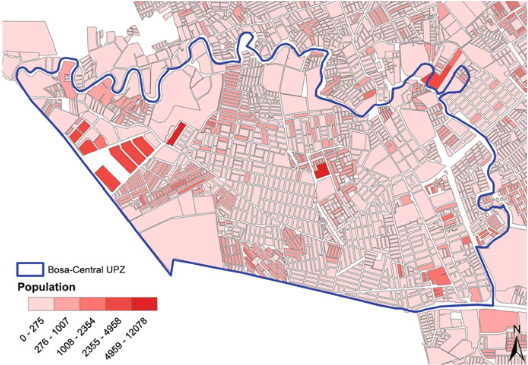
\includegraphics[width=14em]{images/pop-distrib.png}\end{center}}

\begin{frame}{Objective Functions}
\begin{itemize}[<+- | alert@+>]
\item[] \begin{equation*}
\textrm{max } f_1 = \sum_{j \in \mathcal{J}} z_j
\end{equation*}
\item[] \begin{equation*}
\textrm{max } f_2 = \sum_{i \in \mathcal{I}}  \left( \sum_{\{k \in \mathcal{E_P}: d_{ik} \leq r^e  \}} \left( 1-\frac{d_{ik}}{r^e} \right) y_i  -   \sum_{\{k \in \mathcal{E_N}: d_{ik} \leq r^e  \}} \left( 1-\frac{d_{ik}}{r^e} \right) y_i   \right)
\end{equation*}
\item[] \begin{equation*}
\textrm{max } f_3 = \sum_{i \in \mathcal{I}} p_iy_i
\end{equation*}
\item[] \begin{equation*}
\textrm{max } f_4 = \sum_{i \in \mathcal{I}} v_iy_i
\end{equation*}
\item[] \begin{equation*}
\textrm{max } f_5 = \sum_{i \in \mathcal{I}} e_iy_i
\end{equation*}
\item[] \begin{equation*}
\textrm{min } f_6 = \sum_{i \in \mathcal{I}} (c_i^l + c_i^b)y_i
\end{equation*}
\end{itemize}
\end{frame}

\plain{Bogot\'{a}, Colombia}{\vspace{-2em}\begin{center}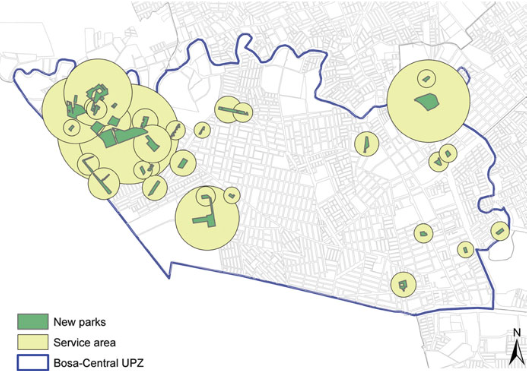
\includegraphics[width=14em]{images/final-sol.png}\end{center}}


\section{The Conclusion}

\begin{frame}[fragile]
\frametitle{Key points}
\begin{itemize}[<+- | alert@+>]
\item Park location case study
\item Community Based Operations Research
\item Linear program
\item Multiobjective problem
\item Worked through an example
\item Solutions
\item Difficult process! 
\end{itemize}

\end{frame}

\section{The End}
\plain{}{Questions?}
\end{document}